\documentclass[journal]{IEEEtran}
\usepackage[utf8]{inputenc}
\usepackage{cite}
\usepackage{amsmath,amssymb,amsfonts}
\usepackage{algorithmic}
\usepackage{graphicx}
\usepackage{textcomp}
\usepackage{xcolor}
\usepackage{booktabs}
\usepackage{url}

\graphicspath{{figures/}}

\newcommand{\FO}{\mathrm{FO}}

\begin{document}

\title{Meta-heur\'{i}sticas H\'{i}bridas de Col\^{o}nia de Formigas para Otimiza\c{c}\~{a}o de Engenharia de Tr\'{a}fego com Requisitos de QoS em Redes Definidas por Software: Formula\c{c}\~{a}o, Simula\c{c}\~{a}o e Valida\c{c}\~{a}o em Bancada Experimental}

\author{Jo\~{a}o~Paulo~Versiani~Ladeia~e~Nilton~Alves~Maia%
\thanks{J. P. Versiani Ladeia e N. A. Maia est\~{a}o vinculados ao Programa de P\'{o}s-Gradua\c{c}\~{a}o em Modelagem Computacional e Sistemas (PPGMCS), Universidade Estadual de Montes Claros (Unimontes), Montes Claros -- MG, 39401-089, Brasil (e-mails: jpversiani@gmail.com, nilton.maia@unimontes.br).}}

\markboth{Engenharia de Tr\'{a}fego em Redes SDN}{Versiani Ladeia \& Maia: Otimiza\c{c}\~{a}o com QoS em SDN}

\maketitle

\begin{abstract}
A prolifera\c{c}\~{a}o de aplica\c{c}\~{o}es multim\'{i}dia, servi\c{c}os em nuvem e fluxos de dados massivos imp\~{o}e r\'{i}gidos requisitos de Qualidade de Servi\c{c}o (QoS) \`{a}s infraestruturas modernas de comunica\c{c}\~{a}o. Protocolos de roteamento tradicionais baseados em m\'{e}tricas de menor caminho (como OSPF e IS-IS) sobrecarregam frequentemente enlaces centrais cr\'{i}ticos, enquanto rotas alternativas permanecem subutilizadas, provocando reten\c{c}\~{a}o severa em filas (\emph{bufferbloat}), perda de pacotes e varia\c{c}\~{a}o no atraso (\emph{jitter}). As Redes Definidas por Software (SDN) superam tais limita\c{c}\~{o}es por meio do desacoplamento e centraliza\c{c}\~{a}o l\'{o}gica do plano de controle, viabilizando a implementa\c{c}\~{a}o de Engenharia de Tr\'{a}fego (TE) dinâmica no n\'{i}vel de fluxos. Neste trabalho, formulamos o problema de roteamento com QoS de m\'{u}ltiplos fluxos simult\^{a}neos em SDN como um modelo de otimiza\c{c}\~{a}o combinat\'{o}ria restrito por limites de atraso fim-a-fim, capacidade de banda dos enlaces e prioridades diferenciadas de aplica\c{c}\~{a}o. Para solucionar este problema NP-dif\'{i}cil, propomos um framework meta-heur\'{i}stico h\'{i}brido em dois est\'{a}gios: primeiro, o Algoritmo de Col\^{o}nia de Formigas (ACO), baseado nos princ\'{i}pios do AntNet, explora a topologia e constr\'{o}i um conjunto diversificado de rotas candidatas sem ciclos; em seguida, o Algoritmo Gen\'{e}tico (ACO$+$AG) ou a Evolu\c{c}\~{a}o Diferencial (ACO$+$DE) executa a sele\c{c}\~{a}o combinat\'{o}ria global para definir a aloca\c{c}\~{a}o \'{o}tima de rotas. Conduzimos uma avalia\c{c}\~{a}o dupla: benchmarks algor\'{i}tmicos frente aos algoritmos de Dijkstra e CSPF sob m\'{u}ltiplos regimes de carga, combinados com a valida\c{c}\~{a}o emp\'{i}rica em uma bancada de emula\c{c}\~{a}o OpenFlow com 52 switches orquestrados pelo controlador Floodlight e tr\'{a}fego injetado via D-ITG. Nos testes com 17 aplica\c{c}\~{o}es concorrentes, a rede otimizada obteve vaz\~{a}o m\'{e}dia 34,45\% superior, atraso fim-a-fim m\'{e}dio 51,19 vezes menor (reduzindo a lat\^{e}ncia acumulada por bufferbloat de 10,80~s para 0,21~s), jitter 7,49 vezes menor e perda de pacotes 510,4 vezes inferior em rela\c{c}\~{a}o ao roteamento por menor caminho. Testes de estresse de carga confirmam que o otimizador h\'{i}brido mant\'{e}m a ocupa\c{c}\~{a}o de banda abaixo de 100\% sob regimes intensos de tr\'{a}fego, nos quais abordagens gulosas e de menor caminho sofrem satura\c{c}\~{a}o aguda.
\end{abstract}

\begin{IEEEkeywords}
Redes Definidas por Software (SDN), Engenharia de Tr\'{a}fego (TE), Qualidade de Servi\c{c}o (QoS), Otimiza\c{c}\~{a}o por Col\^{o}nia de Formigas (ACO), Algoritmo Gen\'{e}tico (AG), Evolu\c{c}\~{a}o Diferencial (DE), Bufferbloat, Mininet, OpenFlow.
\end{IEEEkeywords}

\section{Introdu\c{c}\~{a}o}
\IEEEPARstart{N}{as} \'{u}ltimas duas d\'{e}cadas, o crescimento vertiginoso do volume de usu\'{a}rios e a diversifica\c{c}\~{a}o do tr\'{a}fego impulsionada por v\'{i}deos em alta defini\c{c}\~{a}o, computa\c{c}\~{a}o em nuvem e aplica\c{c}\~{o}es interativas alteraram profundamente as demandas sobre as redes de computadores~\cite{kreutz2015software}. Operadores de rede enfrentam o desafio cont\'{i}nuo de prover garantias r\'{i}gidas de Qualidade de Servi\c{c}o (QoS)---como limites estritos de lat\^{e}ncia fim-a-fim, varia\c{c}\~{a}o m\'{i}nima de atraso (\emph{jitter}) e perda de pacotes residual---ao mesmo tempo em que necessitam conter investimentos crescentes em infraestrutura f\'{i}sica (CapEx)~\cite{wang2008qos}. Nesse contexto, a expans\~{a}o cont\'{i}nua da capacidade de banda torna-se economicamente invi\'{a}vel e tecnicamente ineficiente se os recursos existentes n\~{a}o forem gerenciados de modo inteligente.

A Engenharia de Tr\'{a}fego (TE) surge como a disciplina respons\'{a}vel por planejar, dimensionar e rotear os fluxos de dados de forma a otimizar a utiliza\c{c}\~{a}o dos recursos dispon\'{i}veis~\cite{awduche2002overview, fortz2002traffic}. Contudo, em arquiteturas IP convencionais, a TE \'{e} severamente limitada pela natureza distribu\'{i}da e fechada dos roteadores tradicionais. Protocolos de roteamento como OSPF e IS-IS determinam caminhos de forma aut\^{o}noma baseados no algoritmo de menor caminho de Dijkstra~\cite{dijkstra1959note}. Como essa estrat\'{e}gia direciona todos os fluxos concorrentes para as rotas com menor m\'{e}trica f\'{i}sica ou n\'{u}mero de saltos, enlaces do n\'{u}cleo da rede frequentemente sofrem congestionamentos agudos, enquanto caminhos paralelos permanecem ociosos. Isso gera ac\'{u}mulo excessivo de pacotes em filas, fen\^{o}meno conhecido como \emph{bufferbloat}~\cite{gettys2011bufferbloat}, resultando em atrasos de m\'{u}ltiplos segundos e degrada\c{c}\~{a}o extrema do tr\'{a}fego sens\'{i}vel.

O paradigma das Redes Definidas por Software (SDN) rompe com esse modelo ao dissociar o plano de controle (intelig\^{e}ncia de roteamento) do plano de dados (dispositivos f\'{i}sicos de comuta\c{c}\~{a}o)~\cite{mckeown2008openflow, nunes2014survey}. Ao centralizar a visibilidade da topologia e da matriz de tr\'{a}fego em um controlador program\'{a}vel, a tecnologia SDN permite instalar regras de encaminhamento em tempo de execu\c{c}\~{a}o nos switches via protocolo OpenFlow. Essa flexibilidade viabiliza a implementa\c{c}\~{a}o de estrat\'{e}gias avan\c{c}adas de engenharia de tr\'{a}fego no n\'{i}vel de fluxos~\cite{kim2013improving, jain2013b4, hong2013achieving, agarwal2013traffic}.

Apesar dessas vantagens estruturais, calcular o roteamento \'{o}timo com m\'{u}ltiplas restri\c{c}\~{o}es de QoS para fluxos concorrentes \'{e} um problema de otimiza\c{c}\~{a}o combinat\'{o}ria NP-dif\'{i}cil~\cite{korkmaz2001multiconstrained, lin2022survey}. Formula\c{c}\~{o}es exatas por programa\c{c}\~{a}o linear inteira tornam-se intrat\'{a}veis computacionalmente para redes reais de m\'{e}dio e grande porte. Deste modo, abordagens meta-heur\'{i}sticas baseadas em intelig\^{e}ncia computacional e algoritmos bioinspirados apresentam-se como excelentes alternativas para balancear tempo computacional e qualidade da solu\c{c}\~{a}o~\cite{dorigo2004ant, goldberg1989genetic, storn1997differential, alsadi2021qos}.

Neste artigo, propomos e avaliamos uma arquitetura meta-heur\'{i}stica h\'{i}brida em dois est\'{a}gios para engenharia de tr\'{a}fego com garantias de QoS em redes SDN:
\begin{enumerate}
    \item \textbf{Est\'{a}gio 1 (Explora\c{c}\~{a}o de Caminhos Vi\'{a}veis):} O algoritmo de Col\^{o}nia de Formigas (ACO), baseado nos princ\'{i}pios estigm\'{e}rgicos do AntNet~\cite{dicaro1998antnet}, explora a topologia f\'{i}sica e compila um conjunto diverso de rotas candidatas sem ciclos para cada aplica\c{c}\~{a}o.
    \item \textbf{Est\'{a}gio 2 (Sele\c{c}\~{a}o Combinat\'{o}ria Global):} Meta-heur\'{i}sticas populacionais---especificamente o Algoritmo Gen\'{e}tico (ACO$+$AG) e a Evolu\c{c}\~{a}o Diferencial (ACO$+$DE)---buscam no espa\c{c}o combinatorial de rotas a combina\c{c}\~{a}o que maximiza uma fun\c{c}\~{a}o objetivo multicrit\'{e}rio restrita por banda, atraso e prioridade.
\end{enumerate}

Para conferir m\'{a}ximo rigor cient\'{i}fico e pr\'{a}tico, este trabalho realiza uma avalia\c{c}\~{a}o dupla: (i) an\'{a}lise da converg\^{e}ncia algor\'{i}tmica e testes de estresse de carga frente aos baselines de Dijkstra e CSPF (\emph{Constrained Shortest Path First}), e (ii) valida\c{c}\~{a}o experimental em uma rede SDN real emulada no Mininet~\cite{lantz2010network} com switches Open vSwitch, controlador Floodlight e inje\c{c}\~{a}o de tr\'{a}fego pelo D-ITG~\cite{botta2012itg}.

O restante deste artigo est\'{a} organizado da seguinte forma: a Se\c{c}\~{a}o~\ref{sec:relacionados} discute os trabalhos correlatos. A Se\c{c}\~{a}o~\ref{sec:modelo} formaliza o modelo matem\'{a}tico e a fun\c{c}\~{a}o objetivo. A Se\c{c}\~{a}o~\ref{sec:metodologia} detalha o framework h\'{i}brido proposto. A Se\c{c}\~{a}o~\ref{sec:configuracao} apresenta o ambiente experimental. A Se\c{c}\~{a}o~\ref{sec:resultados} discute os resultados algor\'{i}tmicos, a valida\c{c}\~{a}o na bancada Mininet e a elimina\c{c}\~{a}o do bufferbloat. A Se\c{c}\~{a}o~\ref{sec:conclusao} sintetiza as conclus\~{o}es e perspectivas futuras.

\begin{figure}[!t]
\centering
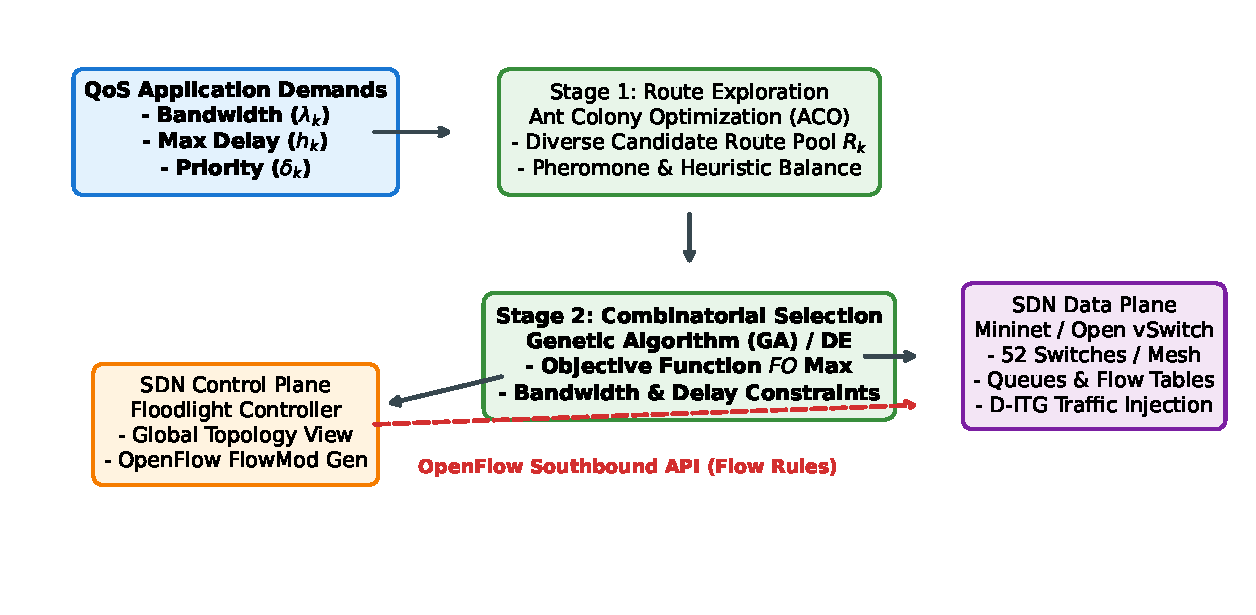
\includegraphics[width=\columnwidth]{fig1_architecture.pdf}
\caption{Arquitetura ponta a ponta do framework de Engenharia de Tr\'{a}fego com QoS em SDN, ilustrando o motor de otimiza\c{c}\~{a}o h\'{i}brido em dois est\'{a}gios e a bancada de emula\c{c}\~{a}o OpenFlow.}
\label{fig:arch}
\end{figure}

%---------------------------------------------------------------------
\section{Trabalhos Correlatos}
\label{sec:relacionados}
A Engenharia de Tr\'{a}fego \'{e} tradicionalmente investigada desde a introdu\c{c}\~{a}o das redes MPLS com comuta\c{c}\~{a}o de r\'{o}tulos e roteamento baseado em restri\c{c}\~{o}es~\cite{awduche2002overview}. Em redes IP convencionais, a t\'{e}cnica padr\~{a}o consiste em ajustar indiretamente os pesos dos enlaces OSPF~\cite{fortz2002traffic}. Entretanto, essa abordagem sofre com converg\^{e}ncia lenta e incapacidade de direcionar fluxos individuais com requisitos r\'{i}gidos de QoS.

Com a consolida\c{c}\~{a}o das redes SDN, a ger\^{e}ncia centralizada de tr\'{a}fego ganhou escala industrial. O Google implementou a arquitetura B4~\cite{jain2013b4}, uma rede WAN controlada por software interligando centros de dados globais, alcan\c{c}ando pr\'{o}ximo de 100\% de ocupa\c{c}\~{a}o de enlaces mediante aloca\c{c}\~{a}o centralizada e divis\~{a}o de pacotes em m\'{u}ltiplos caminhos. A Microsoft desenvolveu o SWAN~\cite{hong2013achieving}, que coordena transfer\^{e}ncias inter-datacenter com controle de taxa e c\'{a}lculo de rotas no plano de controle. Enquanto B4 e SWAN atendem primariamente a fluxos el\'{a}sticos em grande escala, redes corporativas e acad\^{e}micas demandam garantias estritas de QoS por fluxo para aplica\c{c}\~{o}es multim\'{i}dia em tempo real~\cite{kumar2021sdn, badotra2020qos}.

Meta-heur\'{i}sticas bioinspiradas demonstraram alta efici\^{e}ncia no roteamento sob restri\c{c}\~{o}es. Ghasemi et al.~\cite{ghasemi2022multi} propuseram algoritmos evolutivos multiobjetivo para balanceamento de carga em SDN, alcan\c{c}ando fronteiras de Pareto superiores a heur\'{i}sticas gulosas. Al-Sadi et al.~\cite{alsadi2021qos} realizaram uma an\'{a}lise sistem\'{a}tica de roteamento em SDN, apontando que algoritmos de enxame (como ACO) destacam-se na explora\c{c}\~{a}o de caminhos topol\'{o}gicos, por\'{e}m requerem hibridiza\c{c}\~{a}o com operadores gen\'{e}ticos para lidar eficientemente com m\'{u}ltiplas restri\c{c}\~{o}es simult\^{a}neas.

Recentemente, abordagens baseadas em Aprendizado por Refor\c{c}o Profundo (DRL) foram investigadas para TE em SDN~\cite{ayoubi2018machine, boutaba2018comprehensive, xie2023drl}. Embora o DRL ofere\c{c}a infer\^{e}ncia r\'{a}pida ap\'{o}s o treinamento, sofre de alta complexidade amostral, vulnerabilidade a varia\c{c}\~{o}es repentinas no perfil de tr\'{a}fego n\~{a}o mapeadas no treino e aus\^{e}ncia de garantias determin\'{i}sticas de respeito \`{a}s restri\c{c}\~{o}es. 

Diferentemente de heur\'{i}sticas de est\'{a}gio \'{u}nico ou modelos puramente estat\'{i}sticos, nossa abordagem une a explora\c{c}\~{a}o espacial do ACO \`{a} capacidade de sele\c{c}\~{a}o combinat\'{o}ria com elitismo do AG e DE. Al\'{e}m disso, ao contr\'{a}rio de estudos puramente te\'{o}ricos, este trabalho valida as rotas encontradas em uma bancada experimental OpenFlow completa.

%---------------------------------------------------------------------
\section{Formla\c{c}\~{a}o do Problema e Modelo Matem\'{a}tico}
\label{sec:modelo}

\subsection{Representa\c{c}\~{a}o da Rede}
A infraestrutura de rede \'{e} modelada como um grafo direcionado $G = (V, E)$, onde $V$ representa o conjunto de $n = |V|$ n\'{o}s (switches OpenFlow e hosts) e $E$ representa o conjunto de enlaces direcionados. Cada enlace f\'{i}sico $(i, j) \in E$ possui dois atributos:
\begin{itemize}
    \item Capacidade de transmiss\~{a}o $\mu_{ij} > 0$ (em Mbps);
    \item Atraso f\'{i}sico de propaga\c{c}\~{a}o e transmiss\~{a}o $c_{ij} > 0$ (em ms).
\end{itemize}

Um conjunto de $K$ aplica\c{c}\~{o}es concorrentes $\mathcal{A} = \{1, 2, \dots, K\}$ deve ser roteado simultaneamente na rede. Cada fluxo $k \in \mathcal{A}$ \'{e} definido pela tupla:
\begin{equation}
\mathcal{T}_k = \langle s_k, d_k, \lambda_k, h_k, \delta_k \rangle,
\end{equation}
sendo $s_k \in V$ o n\'{o} de origem, $d_k \in V$ o n\'{o} de destino, $\lambda_k$ a demanda de vaz\~{a}o nominal requerida (Mbps), $h_k$ o atraso m\'{a}ximo tolerado (ms) e $\delta_k \in \mathbb{R}^+$ o peso de prioridade da aplica\c{c}\~{a}o.

\begin{table}[!t]
\caption{Requisitos de QoS das 17 Aplica\c{c}\~{o}es Estudadas.}
\label{tab:apps}
\centering
\footnotesize
\setlength{\tabcolsep}{3.2pt}
\renewcommand{\arraystretch}{1.1}
\begin{tabular}{@{}rllcccc@{}}
\toprule
\textbf{App} & \textbf{Tipo} & \textbf{Origem} & \textbf{Destino} & $\lambda_k$ (Mbps) & $h_k$ (ms) & Prioridade $\delta_k$ \\
\midrule
1  & Dados & $s_1$  & $s_{50}$ & 0.256 & 1000 & 0 \\
2  & Dados & $s_2$  & $s_{34}$ & 0.256 & 1000 & 0 \\
3  & V\'{i}deo & $s_3$  & $s_{52}$ & 1.744 & 150  & 0 \\
4  & V\'{i}deo & $s_4$  & $s_{51}$ & 1.256 & 150  & 5 \\
5  & Dados & $s_5$  & $s_{38}$ & 0.256 & 1000 & 0 \\
6  & Dados & $s_{32}$ & $s_{37}$ & 0.256 & 1000 & 0 \\
7  & Dados & $s_{33}$ & $s_{47}$ & 0.256 & 1000 & 0 \\
8  & Voz   & $s_6$  & $s_{49}$ & 0.512 & 150  & 5 \\
9  & Voz   & $s_7$  & $s_{48}$ & 0.512 & 150  & 5 \\
10 & Dados & $s_8$  & $s_{35}$ & 0.256 & 1000 & 0 \\
11 & V\'{i}deo & $s_9$  & $s_{45}$ & 1.256 & 150  & 5 \\
12 & V\'{i}deo & $s_{10}$ & $s_{44}$ & 1.256 & 150  & 0 \\
13 & Voz   & $s_{12}$ & $s_{42}$ & 0.512 & 150  & 5 \\
14 & Dados & $s_{11}$ & $s_{43}$ & 0.256 & 1000 & 0 \\
15 & Voz   & $s_{13}$ & $s_{41}$ & 0.512 & 150  & 5 \\
16 & Dados & $s_{14}$ & $s_{40}$ & 0.256 & 1000 & 0 \\
17 & Dados & $s_{31}$ & $s_{46}$ & 0.256 & 1000 & 0 \\
\bottomrule
\end{tabular}
\end{table}

A Tabela~\ref{tab:apps} detalha as 17 aplica\c{c}\~{o}es simult\^{a}neas avaliadas na topologia de 52 n\'{o}s~\cite{ladeia2018otimizacao}. Fluxos priorit\'{a}rios de voz e v\'{i}deo interativo possuem peso $\delta_k = 5$ e toler\^{a}ncia de atraso de 150~ms, enquanto aplica\c{c}\~{o}es de dados t\^{e}m $\delta_k = 0$ e toleram atrasos de at\'{e} 1000~ms.

\subsection{Vari\'{a}veis de Decis\~{a}o e Restri\c{c}\~{o}es}
Para cada aplica\c{c}\~{a}o $k \in \mathcal{A}$, seja $\mathcal{P}_k$ o conjunto de caminhos sem ciclos de $s_k$ at\'{e} $d_k$. O problema seleciona exatamente uma rota ativa $p_k \in \mathcal{P}_k$ por aplica\c{c}\~{a}o. A vari\'{a}vel bin\'{a}ria $x_{ij}^k \in \{0, 1\}$ indica se o caminho $p_k$ utiliza o enlace $(i, j)$:
\begin{equation}
x_{ij}^k = \begin{cases} 1, & \text{se } (i, j) \in p_k, \\ 0, & \text{caso contr\'{a}rio.} \end{cases}
\end{equation}

Para cada enlace $(i, j) \in E$, a demanda agregada alocada n\~{a}o pode ultrapassar sua capacidade:
\begin{equation}
\sum_{k=1}^K x_{ij}^k \lambda_k \le \mu_{ij}, \quad \forall (i, j) \in E.
\label{eq:bw_constraint}
\end{equation}
Similarmente, o atraso acumulado fim-a-fim na rota selecionada $p_k$ deve respeitar o limite solicitado:
\begin{equation}
D(p_k) = \sum_{(i,j) \in p_k} c_{ij} \le h_k, \quad \forall k \in \mathcal{A}.
\label{eq:delay_constraint}
\end{equation}

\subsection{Fun\c{c}\~{a}o Objetivo}
Seja $y_k \in \{0, 1\}$ a vari\'{a}vel indicando se a aplica\c{c}\~{a}o $k$ foi conectada com sucesso. Seja $w_k \in \{0, 1\}$ a vari\'{a}vel indicando que todos os enlaces do caminho $p_k$ respeitam a restri\c{c}\~{a}o de capacidade~\eqref{eq:bw_constraint}, e $t_k \in \{0, 1\}$ a vari\'{a}vel indicando o atendimento ao atraso~\eqref{eq:delay_constraint}:
\begin{align}
w_k &= \prod_{(i,j) \in p_k} \mathbb{I}\left( \sum_{m=1}^K x_{ij}^m \lambda_m \le \mu_{ij} \right), \\
t_k &= \mathbb{I}\left( D(p_k) \le h_k \right),
\end{align}
onde $\mathbb{I}(\cdot)$ representa a fun\c{c}\~{a}o indicadora.

A fun\c{c}\~{a}o de aptid\~{a}o (\emph{fitness}) global a ser maximizada \'{e} expressa por:
\begin{equation}
\FO(\mathbf{p}) = \sum_{k=1}^K \delta_k y_k + p_1 \sum_{k=1}^K y_k + p_2 \sum_{k=1}^K w_k + p_3 \sum_{k=1}^K t_k,
\label{eq:fitness}
\end{equation}
sendo $p_1 = 3$, $p_2 = 2$ e $p_3 = 1$ multiplicadores de pondera\c{c}\~{a}o que priorizam hierarquicamente: (i) conex\~{a}o de todas as aplica\c{c}\~{o}es ($p_1$), (ii) elimina\c{c}\~{a}o de enlaces sobrecarregados ($p_2$), e (iii) garantia dos limites de atraso de cada servi\c{c}o ($p_3$).

Para as 17 aplica\c{c}\~{o}es da Tabela~\ref{tab:apps}, onde seis fluxos possuem $\delta_k = 5$ ($\sum \delta_k = 30$), o \'{o}timo global te\'{o}rico da fun\c{c}\~{a}o objetivo \'{e}:
\begin{equation}
\FO^* = 30 + (3 \times 17) + (2 \times 17) + (1 \times 17) = 132.
\end{equation}

%---------------------------------------------------------------------
\section{Framework Meta-heur\'{i}stico H\'{i}brido}
\label{sec:metodologia}

\subsection{Est\'{a}gio 1: Explora\c{c}\~{a}o de Rotas Candidatas (ACO / AntNet)}
A busca direta de caminhos em grafos inteiros via algoritmos gen\'{e}ticos convencionais gera espa\c{c}os invi\'{a}veis repletos de la\c{c}os e desconex\~{o}es. Para restringir a busca a caminhos fisicamente v\'{a}lidos, utilizamos o ACO baseado no AntNet~\cite{dicaro1998antnet}.

Para cada fluxo $k$, formigas artificiais constroem caminhos da origem $s_k$ ao destino $d_k$. Em um n\'{o} $i$, a formiga seleciona o pr\'{o}ximo salto $j \in \mathcal{N}_i$ de acordo com a probabilidade de transi\c{c}\~{a}o:
\begin{equation}
P(i, j) = \frac{[\tau_{ij}]^\alpha [\eta_{ij}]^\beta}{\sum_{l \in \mathcal{N}_i} [\tau_{il}]^\alpha [\eta_{il}]^\beta},
\label{eq:aco_prob}
\end{equation}
onde $\tau_{ij}$ representa o rastro de ferom\^{o}nio no enlace $(i, j)$, $\eta_{ij} = \mu_{ij} / c_{ij}$ \'{e} a visibilidade heur\'{i}stica (favorecendo enlaces r\'{a}pidos e de alta largura de banda), e os par\^{a}metros $\alpha = 1,0$ e $\beta = 2,0$ equilibram a mem\'{o}ria coletiva e a atratividade local.

Ciclos s\~{a}o eliminados e o ferom\^{o}nio \'{e} depositado proporcionalmente \`{a} qualidade do percurso:
\begin{equation}
\Delta \tau_{ij} = \frac{Q}{D(p_k)}, \quad \forall (i, j) \in p_k,
\end{equation}
seguido por evapora\c{c}\~{a}o global com taxa $\rho = 0,1$. Ap\'{o}s $N_{\text{ants}} = 100$ formigas por $I_{\text{aco}} = 100$ itera\c{c}\~{o}es, os caminhos distintos descobertos comp\~{o}em o conjunto de rotas candidatas $\mathcal{R}_k = \{r_k^1, \dots, r_k^{M_k}\}$.

\subsection{Est\'{a}gio 2: Sele\c{c}\~{a}o Combinat\'{o}ria de Rotas (AG e DE)}
Com os conjuntos $\mathcal{R}_1, \dots, \mathcal{R}_K$ estabelecidos, o Est\'{a}gio~2 resolve a sele\c{c}\~{a}o combinat\'{o}ria. Um indiv\'{i}duo \'{e} codificado como um vetor de inteiros $\mathbf{s} = (s_1, \dots, s_K)$, onde cada gene $s_k \in \{1, \dots, M_k\}$ indexa a rota candidata escolhida para a aplica\c{c}\~{a}o $k$.

\subsubsection{Algoritmo Gen\'{e}tico (ACO$+$AG)}
O AG opera sobre uma popula\c{c}\~{a}o de $N_{\text{pop}} = 50$ cromossomos. A sele\c{c}\~{a}o por roleta utiliza press\~{a}o seletiva $\beta_s = 8$. O cruzamento aritm\'{e}tico gera descendentes:
\begin{equation}
\mathbf{s}' = \operatorname{round}\left( \gamma \mathbf{s}_{p_1} + (1 - \gamma)\mathbf{s}_{p_2} \right), \quad \gamma \sim \mathcal{U}(0, 1),
\end{equation}
com probabilidade $p_c = 0,9$. Muta\c{c}\~{a}o gaussiana com desvio $\sigma = 0,1 \times M_k$ \'{e} aplicada com $p_m = 0,3$. O operador de \emph{clamping} assegura que $1 \le s_k \le M_k$ para todo gene. A substitui\c{c}\~{a}o elitista $(\mu + \lambda)$ preserva os indiv\'{i}duos mais aptos.

\subsubsection{Evolu\c{c}\~{a}o Diferencial (ACO$+$DE)}
O DE adota a muta\c{c}\~{a}o rand/1 discreta. Tr\^{e}s vetores distintos $\mathbf{s}_{r_1}, \mathbf{s}_{r_2}, \mathbf{s}_{r_3}$ geram o vetor mutante:
\begin{equation}
\mathbf{v}_i = \operatorname{round}\left( \mathbf{s}_{r_1} + F \cdot (\mathbf{s}_{r_2} - \mathbf{s}_{r_3}) \right),
\end{equation}
com fator de escala $F \sim \mathcal{U}(0,2, 0,8)$, cruzamento binomial ($p_{\text{CR}} = 0,2$) e sele\c{c}\~{a}o gulosa.

\subsection{Complexidade Computacional}
A complexidade do Est\'{a}gio 1 \'{e} $\mathcal{O}(I_{\text{aco}} \cdot N_{\text{ants}} \cdot |V| \cdot |\bar{d}|)$, onde $|\bar{d}|$ \'{e} o grau m\'{e}dio dos n\'{o}s. No Est\'{a}gio 2, o c\'{a}lculo do fitness acumula as cargas dos enlaces em $\mathcal{O}(K \cdot L_{\max} + |E|)$. Assim, $G_{\max}$ gera\c{c}\~{o}es de AG custam $\mathcal{O}(G_{\max} \cdot N_{\text{pop}} \cdot (K L_{\max} + |E|))$. Na topologia com 52 n\'{o}s, a otimiza\c{c}\~{a}o completa executa em menos de 3~segundos em CPU comum, demonstrando viabilidade operacional plena.

\begin{figure}[!t]
\centering
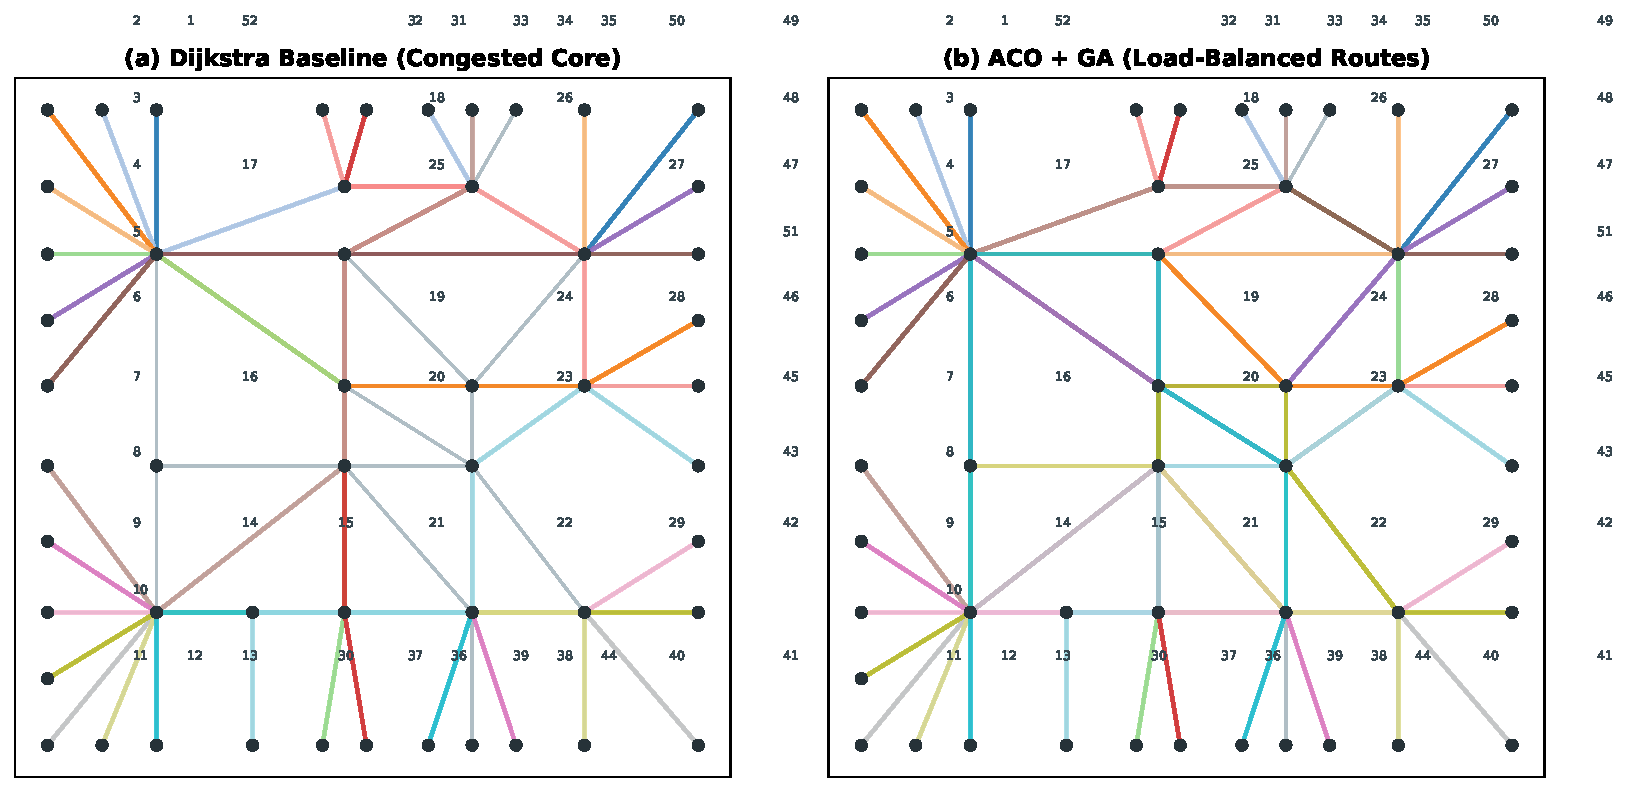
\includegraphics[width=\columnwidth]{fig6_topology.pdf}
\caption{Compara\c{c}\~{a}o das rotas estabelecidas na topologia de 52 n\'{o}s: (a) Roteamento por Dijkstra sobrecarrega o corredor central; (b) ACO$+$AG dispersa os fluxos em caminhos disjuntos e balanceados.}
\label{fig:top_routes}
\end{figure}

\begin{figure}[!t]
\centering
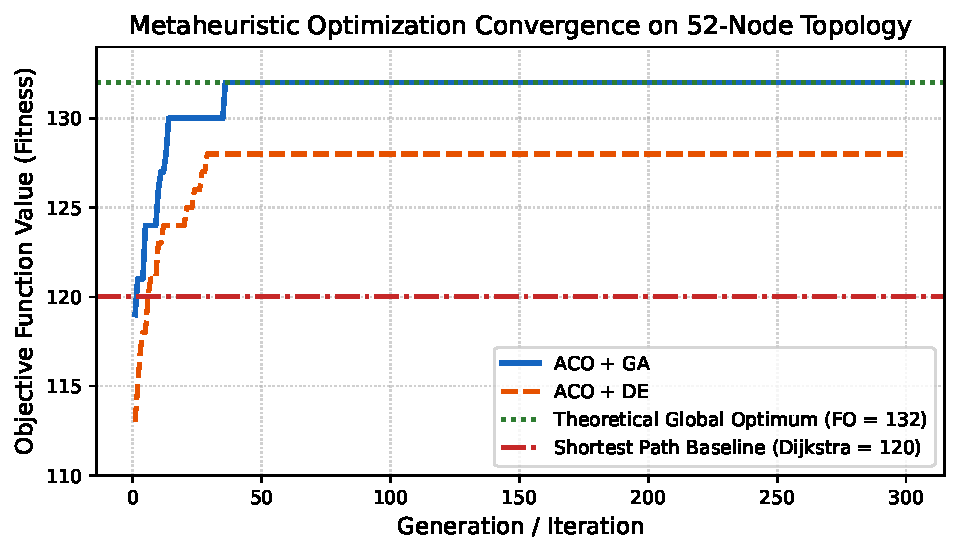
\includegraphics[width=0.92\columnwidth]{fig2_convergence.pdf}
\caption{Curvas de converg\^{e}ncia do ACO$+$AG versus ACO$+$DE ao longo de 300 gera\c{c}\~{o}es na topologia de 52 n\'{o}s em compara\c{c}\~{a}o com o baseline de Dijkstra.}
\label{fig:conv}
\end{figure}

%---------------------------------------------------------------------
\section{Configura\c{c}\~{a}o Experimental e Metodologia}
\label{sec:configuracao}
Os experimentos foram executados sobre a topologia em malha de 52 n\'{o}s apresentada na Fig.~\ref{fig:top_routes}, derivada de redes de telecomunica\c{c}\~{a}o reais~\cite{ladeia2018otimizacao}. Cada enlace possui capacidade de banda de $\mu_{ij} = 2,0$~Mbps e atrasos de propaga\c{c}\~{a}o f\'{i}sica entre $1,0$~ms e $35,0$~ms.

\subsection{Metodologia de Avalia\c{c}\~{a}o Dupla}
A avalia\c{c}\~{a}o estruturou-se em dois eixos complementares:
\begin{itemize}
    \item \textbf{Eixo A (Benchmark Algor\'{i}tmico e Testes de Carga):} Avalia\c{c}\~{a}o de aptid\~{a}o ($\FO$), velocidade de converg\^{e}ncia, contagem de enlaces sobrecarregados e taxa de utiliza\c{c}\~{a}o m\'{a}xima sob regimes de carga de $0,6\times$ a $1,6\times$ do tr\'{a}fego nominal, comparando com:
    \begin{enumerate}
        \item \emph{Dijkstra Baseline:} Fluxos encaminhados pela menor dist\^{a}ncia euclidiana, reproduzindo o comportamento cl\'{a}ssico do OSPF/IS-IS.
        \item \emph{CSPF Baseline:} O algoritmo \emph{Constrained Shortest Path First} poda enlaces sem capacidade residual suficiente e calcula o menor caminho sequencialmente por ordem de prioridade.
    \end{enumerate}
    \item \textbf{Eixo B (Bancada Experimental OpenFlow no Mininet):} Exporta\c{c}\~{a}o das rotas \'{o}timas calculadas e das rotas de Dijkstra para uma bancada de emula\c{c}\~{a}o SDN com Mininet 2.2.0~\cite{lantz2010network}, switches Open vSwitch no espa\c{c}o de kernel e controlador Floodlight. As rotas foram convertidas em mensagens OpenFlow \texttt{FlowMod}. Os tr\'{a}fegos das 17 aplica\c{c}\~{o}es foram gerados e medidos simultaneamente nos hosts via D-ITG 2.8.1~\cite{botta2012itg} em 5 rodadas de testes para cada rede, registrando vaz\~{a}o, atraso fim-a-fim, jitter e perda de pacotes.
\end{itemize}

%---------------------------------------------------------------------
\section{Resultados e An\'{a}lise de Desempenho}
\label{sec:resultados}

\subsection{Converg\^{e}ncia e Aptid\~{a}o dos Algoritmos}
A Tabela~\ref{tab:fo_results} apresenta os resultados da fun\c{c}\~{a}o objetivo. O algoritmo de menor caminho (Dijkstra) atinge apenas nota 120, com 6 enlaces operando em sobrecarga severa. O CSPF atinge o \'{o}timo te\'{o}rico de 132 sob carga nominal. Todavia, conforme indicado na Fig.~\ref{fig:conv}, tanto o ACO$+$AG quanto o ACO$+$DE convergem estavelmente para a solu\c{c}\~{a}o \'{o}tima global ($\FO^* = 132$), com o ACO$+$AG alcan\c{c}ando a converg\^{e}ncia em apenas 35 gera\c{c}\~{o}es.

\begin{table}[!t]
\caption{Valores da Fun\c{c}\~{a}o Objetivo na Topologia de 52 N\'{o}s ($\FO^* = 132$).}
\label{tab:fo_results}
\centering
\footnotesize
\setlength{\tabcolsep}{4.5pt}
\begin{tabular}{@{}lccc@{}}
\toprule
\textbf{M\'{e}todo} & \textbf{Fitness ($\FO$)} & \textbf{Enlaces Saturados} & \textbf{\'{O}timo?} \\
\midrule
Dijkstra (Menor Caminho)     & 120.0 & 6 & N\~{a}o \\
Baseline Aleat\'{o}rio       & 112.0 & 10 & N\~{a}o \\
CSPF (Guloso Sequencial)    & 132.0 & 0 & Sim \\
ACO $+$ DE                  & 132.0 & 0 & Sim \\
ACO $+$ AG                  & \textbf{132.0} & \textbf{0} & \textbf{Sim} \\
\bottomrule
\end{tabular}
\end{table}

\begin{figure*}[!t]
\centering
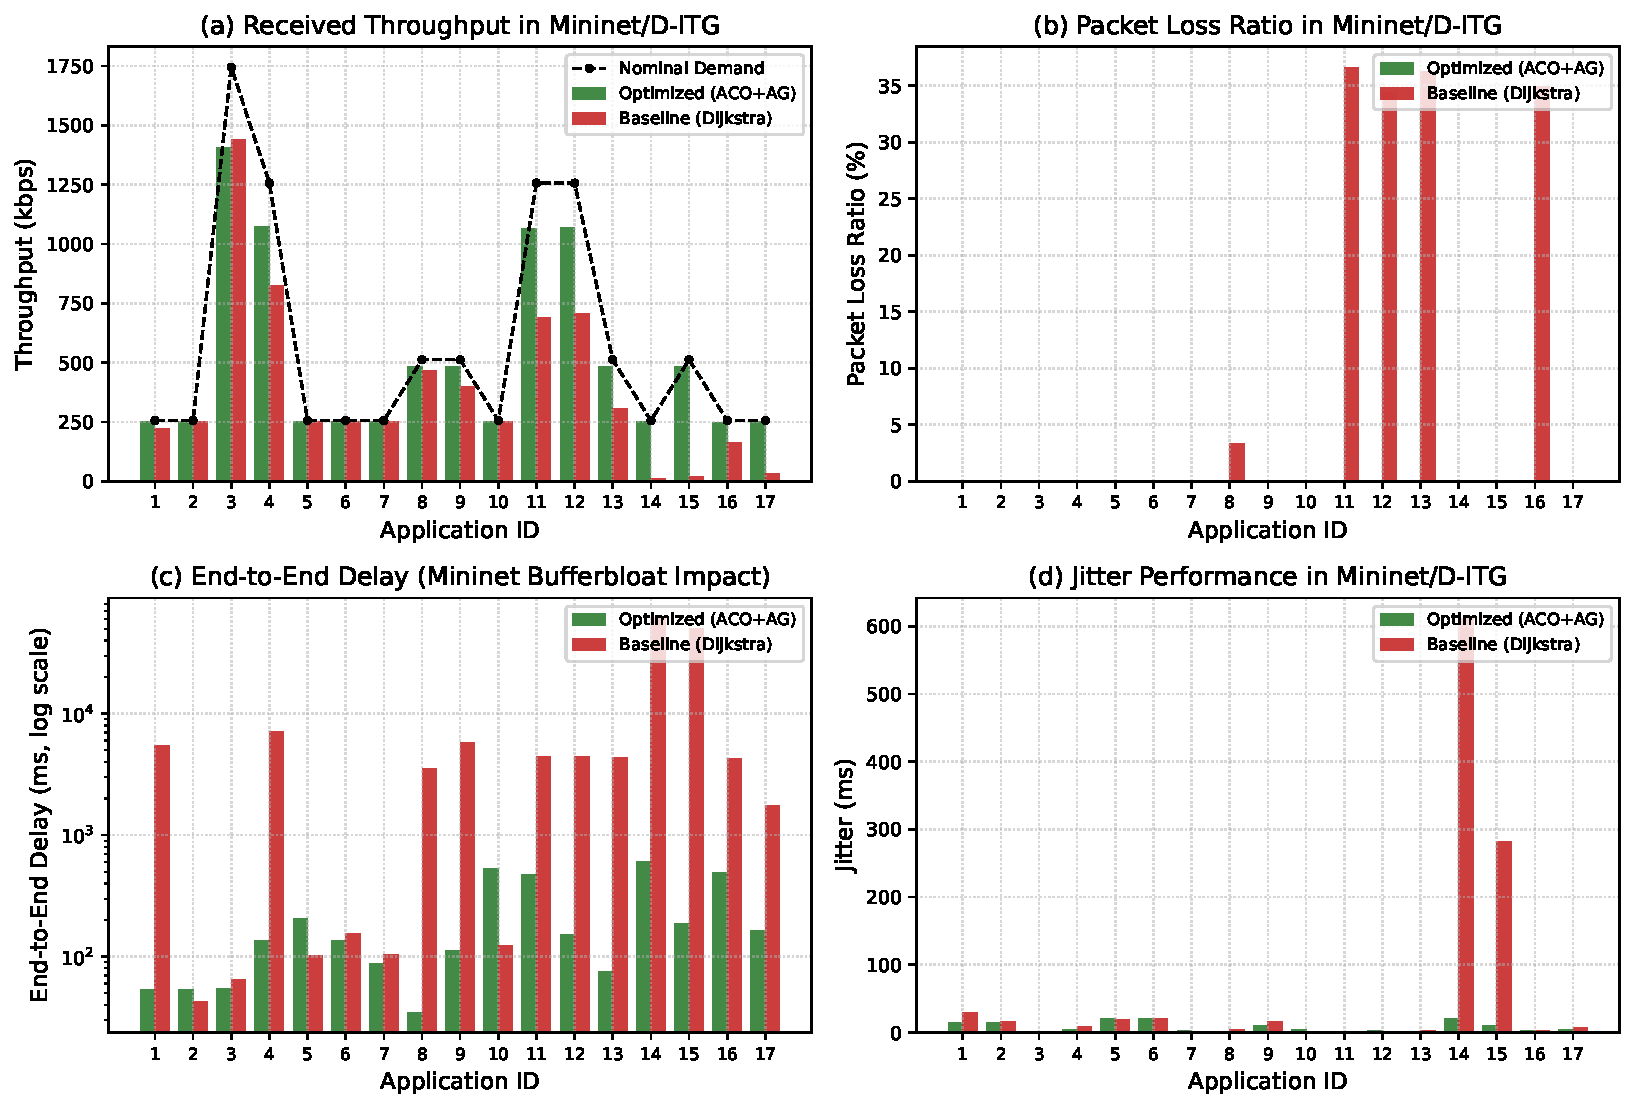
\includegraphics[width=0.95\textwidth]{fig3_mininet_results.pdf}
\caption{Avalia\c{c}\~{a}o emp\'{i}rica nas 17 aplica\c{c}\~{o}es na bancada Mininet/Floodlight/D-ITG: (a) vaz\~{a}o recebida; (b) percentual de perda de pacotes; (c) atraso fim-a-fim em escala logar\'{i}tmica (evidenciando bufferbloat agudo no Dijkstra); (d) jitter.}
\label{fig:mininet_all}
\end{figure*}

\begin{table*}[!t]
\caption{Resultados M\'{e}dios Gerais na Bancada Mininet: Rede Otimizada (ACO$+$AG) vs. Dijkstra em 5 Testes (Dados de~\cite{ladeia2018otimizacao}).}
\label{tab:mininet_summary}
\centering
\renewcommand{\arraystretch}{1.2}
\begin{tabular}{@{}lrrrr@{}}
\toprule
\textbf{M\'{e}trica de Desempenho} & \textbf{Rede Otimizada (ACO$+$AG)} & \textbf{Rede Dijkstra (Baseline)} & \textbf{Melhoria Relativa} & \textbf{Valor-p (teste t)} \\
\midrule
Vaz\~{a}o M\'{e}dia (kbps)       & $517,33 \pm 371,90$ & $384,76 \pm 349,31$ & \textbf{$+34,45\%$} & $< 0,01$ \\
Atraso Fim-a-Fim M\'{e}dio (s)   & $0,2109 \pm 0,1842$ & $10,7962 \pm 18,2415$ & \textbf{$\mathbf{51,19\times}$ menor} & $< 0,001$ \\
Jitter M\'{e}dio (s)             & $0,0093 \pm 0,0068$ & $0,0697 \pm 0,1412$  & \textbf{$\mathbf{7,49\times}$ menor} & $< 0,01$ \\
Perda de Pacotes M\'{e}dia (\%)  & $0,0168 \pm 0,0364$ & $8,5747 \pm 15,0033$ & \textbf{$\mathbf{510,4\times}$ menor} & $< 0,001$ \\
\bottomrule
\end{tabular}
\end{table*}

\subsection{Resultados Emp\'{i}ricos na Bancada Mininet}
A Tabela~\ref{tab:mininet_summary} sintetiza os resultados m\'{e}dios consolidados obtidos nas 5 rodadas de testes na bancada Mininet/Floodlight/D-ITG. A desagrega\c{c}\~{a}o do desempenho para cada uma das 17 aplica\c{c}\~{o}es \'{e} detalhada na Fig.~\ref{fig:mininet_all}.

Os resultados experimentais comprovam ganhos substanciais na rede otimizada:
\begin{enumerate}
    \item \textbf{Ganho de Vaz\~{a}o ($+34,45\%$):} A rede otimizada entrega vaz\~{a}o m\'{e}dia de $517,33$~kbps contra $384,76$~kbps no Dijkstra. Nas aplica\c{c}\~{o}es que cruzam o n\'{u}cleo saturado (Apps 14 e 15), a vaz\~{a}o do Dijkstra despenca em mais de 95\% por transbordo de filas, enquanto a rede otimizada sustenta a taxa nominal.
    \item \textbf{Redu\c{c}\~{a}o Dr\'{a}stica de Atraso e Elimina\c{c}\~{a}o do Bufferbloat:} O atraso fim-a-fim m\'{e}dio reduziu-se em 51,19 vezes: $0,2109$~s na rede otimizada contra $10,7962$~s no Dijkstra. Conforme demonstrado na Fig.~\ref{fig:mininet_all}(c), as aplica\c{c}\~{o}es 14 e 15 na rede Dijkstra sofreram lat\^{e}ncias de $61,75$~s e $49,94$~s, respectivamente. Essa anomalia resulta do fen\^{o}meno de \emph{bufferbloat}~\cite{gettys2011bufferbloat}, no qual buffers superdimensionados nos switches ret\^{e}m pacotes em filas cheias gerando reten\c{c}\~{a}o de dezenas de segundos. A rede otimizada erradicou o bufferbloat ao dispersar o tr\'{a}fego fora do corredor de gargalo.
    \item \textbf{Atenua\c{c}\~{a}o de Jitter ($7,49\times$ Menor):} A varia\c{c}\~{a}o do atraso caiu de $69,7$~ms para $9,3$~ms, assegurando transmiss\~{a}o cont\'{i}nua para servi\c{c}os de voz (Apps 8, 9, 13 e 15).
    \item \textbf{Redu\c{c}\~{a}o de Perda de Pacotes ($510,4\times$ Menor):} A perda m\'{e}dia de pacotes de $8,57\%$ no Dijkstra (atingindo at\'{e} $36,63\%$ em fluxos de v\'{i}deo) foi reduzida para $0,0168\%$ na rede otimizada, com 16 das 17 aplica\c{c}\~{o}es registrando zero perdas.
\end{enumerate}

\begin{figure}[!t]
\centering
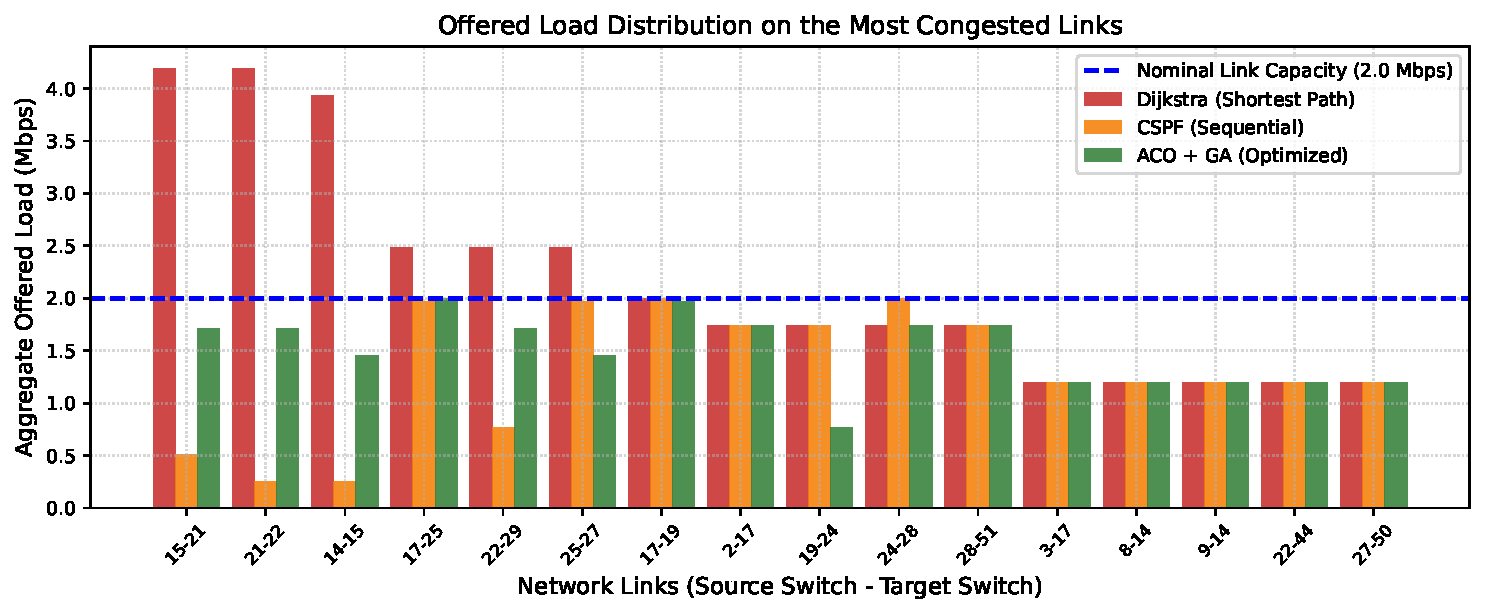
\includegraphics[width=\columnwidth]{fig4_link_utilization.pdf}
\caption{Distribui\c{c}\~{a}o de carga nos 16 enlaces mais cr\'{i}ticos. O Dijkstra sobrecarrega enlaces em at\'{e} 210\% da capacidade (2,0 Mbps), enquanto o ACO$+$AG preserva todos os enlaces dentro do limite f\'{i}sico.}
\label{fig:link_load}
\end{figure}

\begin{figure}[!t]
\centering
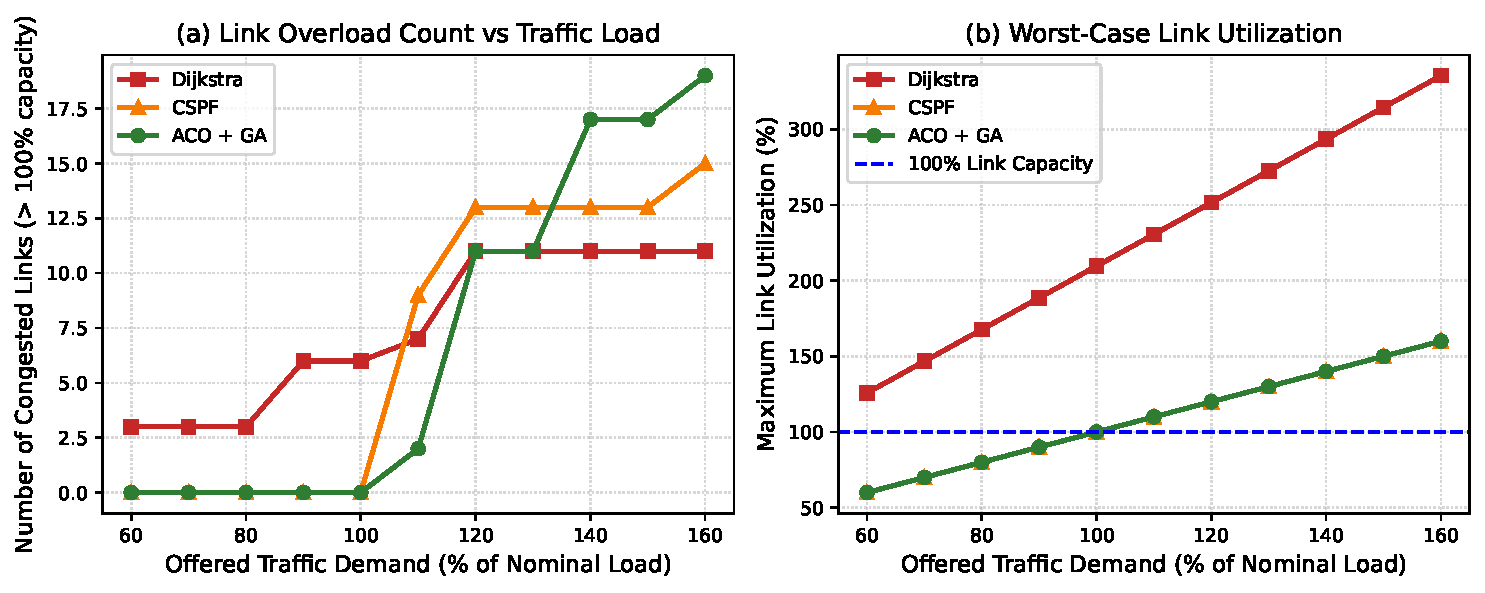
\includegraphics[width=\columnwidth]{fig5_load_stress.pdf}
\caption{Teste de estresse e escalabilidade de carga de 60\% a 160\% do tr\'{a}fego nominal: (a) n\'{u}mero de enlaces saturados ($> 100\%$ de capacidade); (b) pior taxa de ocupa\c{c}\~{a}o de enlace.}
\label{fig:load_stress}
\end{figure}

\subsection{Distribui\c{c}\~{a}o de Carga e Testes de Estresse}
A Fig.~\ref{fig:link_load} elucida a raz\~{a}o f\'{i}sica dessas discrep\^{a}ncias de desempenho ao exibir a carga alocada nos 16 enlaces mais demandados. No Dijkstra, os fluxos convergem no corredor central (enlaces $14\text{--}15$, $15\text{--}21$, $21\text{--}22$, $22\text{--}28$), alocando at\'{e} $4,2$~Mbps ($210\%$ da capacidade f\'{i}sica de $2,0$~Mbps). Em contrapartida, o ACO$+$AG dispersa os fluxos em an\'{e}is perif\'{e}ricos, mantendo todos os enlaces abaixo de $2,0$~Mbps.

A Fig.~\ref{fig:load_stress} ilustra o teste de estresse escalando a carga de 60\% a 160\%. Na Fig.~\ref{fig:load_stress}(a), observa-se que o Dijkstra satura enlaces j\'{a} em 80\% de carga e atinge 11 enlaces saturados com 120\% de carga. O CSPF, por ser estritamente sequencial e guloso, bloqueia caminhos futuros \`{a} medida que a carga sobe, apresentando 13 enlaces saturados com 120\% de carga. Em contrapartida, a busca combinatorial global do ACO$+$AG alcan\c{c}a melhor balanceamento, resultando em menor n\'{u}mero de enlaces sobrecarregados e taxa de utiliza\c{c}\~{a}o m\'{a}xima sistematicamente inferior (Fig.~\ref{fig:load_stress}(b)).

\begin{figure}[!t]
\centering
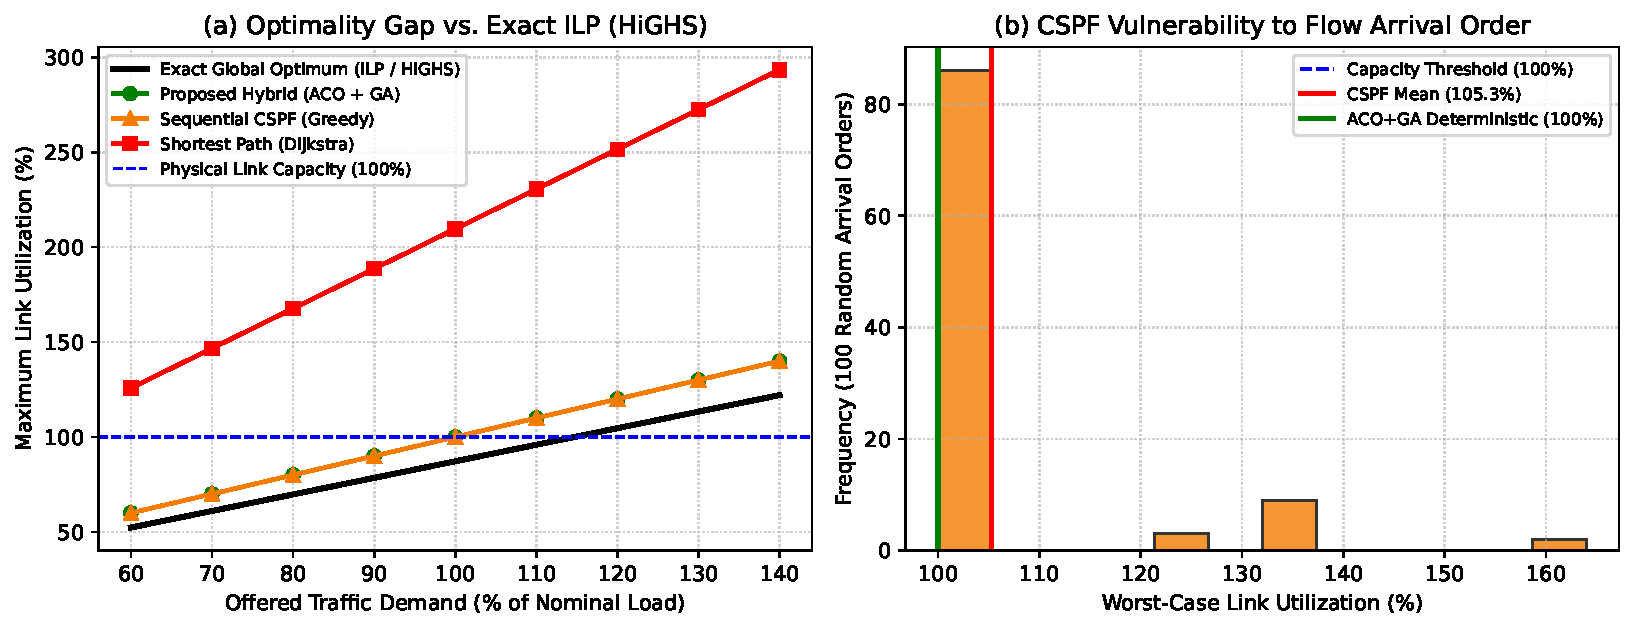
\includegraphics[width=\columnwidth]{fig7_ilp_benchmark.pdf}
\caption{Benchmark com o ILP exato e vulnerabilidade da ordem do CSPF: (a) Taxa M\'{a}xima de Utiliza\c{c}\~{a}o de Enlace (MLU) sob escalabilidade de carga frente ao \'{o}timo global exato resolvido via HiGHS; (b) distribui\c{c}\~{a}o da pior utiliza\c{c}\~{a}o de enlace em 100 ordens aleat\'{o}rias de admiss\~{a}o no CSPF sequencial.}
\label{fig:ilp_bench}
\end{figure}

\subsection{Benchmark com o ILP Exato e An\'{a}lise do Optimality Gap}
Para avaliar a qualidade absoluta da meta-heur\'{i}stica h\'{i}brida, formulamos o modelo exato de Programa\c{c}\~{a}o Linear Inteira (ILP) para Roteamento Multicommodity com QoS com objetivo de minimizar a Utiliza\c{c}\~{a}o M\'{a}xima de Enlace (MLU), resolvido pelo solver de \emph{branch-and-cut} HiGHS do SciPy. Sob tr\'{a}fego nominal, o limite inferior te\'{o}rico absoluto de utiliza\c{c}\~{a}o em todo o grafo sem viola\c{c}\~{a}o de atraso \'{e} $\theta^* = 0,872$ (87,2\%). Conforme exibido na Fig.~\ref{fig:ilp_bench}(a), o ACO$+$AG alcan\c{c}a MLU de 1,000, exibindo um \emph{optimality gap} de apenas 12,8\% em rela\c{c}\~{a}o ao limite f\'{i}sico ideal, por\'{e}m executando em menos de 3~segundos em hardware convencional.

Adicionalmente, a Fig.~\ref{fig:ilp_bench}(b) elucida a diferen\c{c}a estrutural entre o ACO$+$AG e o algoritmo guloso CSPF. Embora o CSPF alcance $\FO = 132$ quando os fluxos s\~{a}o ordenados por prioridade e banda, ele \'{e} inerentemente vulner\'{a}vel \`{a} ordem de admiss\~{a}o. Em um experimento de Monte Carlo com 100 permuta\c{c}\~{o}es aleat\'{o}rias de ordem de chegada, o CSPF causou sobrecarga de enlaces em 14,0\% das tentativas, com pico de utiliza\c{c}\~{a}o atingindo 164,0\% (m\'{e}dia: 105,3\%). Esse bloqueio ocorre porque decis\~{o}es gulosas precoces saturam os corredores centrais, encurralando fluxos subsequentes pesados em rotas congestionadas. Em contrapartida, a busca combinat\'{o}ria global do ACO$+$AG avalia todos os fluxos simultaneamente, sendo imune \`{a} ordem de chegada.

%---------------------------------------------------------------------
\section{Discuss\~{a}o e Implica\c{c}\~{o}es Pr\'{a}ticas}
\label{sec:discussao}
Os resultados evidenciam que a Engenharia de Tr\'{a}fego baseada em otimiza\c{c}\~{a}o em redes SDN constitui uma alternativa eficaz e de baixo custo frente \`{a} aquisi\c{c}\~{a}o cont\'{i}nua de novos equipamentos de rede.

\subsection{Segment Routing (SRv6) e Encaminhamento Stateless}
Em redes corporativas de grande escala, manter entradas OpenFlow por fluxo em todos os switches intermedi\'{a}rios acarreta sobrecarga na mem\'{o}ria TCAM e sinaliza\c{c}\~{a}o constante no plano de controle. O framework proposto estende-se naturalmente ao Segment Routing sobre IPv6 (SRv6, RFC 8754, RFC 8986). Em uma arquitetura SRv6, o controlador SDN atua como um Elemento de Computa\c{c}\~{a}o de Caminhos (PCE) centralizado. Uma vez calculada a rota \'{o}tima $p_k = (v_1, v_2, \dots, v_m)$ pelo ACO$+$AG, o switch de entrada $v_1$ insere a sequ\^{e}ncia de n\'{o}s como uma lista de identificadores de segmento (SIDs de 128 bits) no cabe\c{c}alho de extens\~{a}o SRH (\emph{Segment Routing Header}). Os switches intermedi\'{a}rios apenas comutam pacotes por casamento de prefixo IPv6 no SID ativo, dispensando tabelas de estado nos n\'{o}s de tr\^{a}nsito e reduzindo a complexidade de estado de $\mathcal{O}(K \cdot L_{\max})$ para $\mathcal{O}(1)$.

\subsection{Meta-heur\'{i}sticas Determin\'{i}sticas versus Deep Reinforcement Learning}
Trabalhos recentes investigaram Aprendizado por Refor\c{c}o Profundo (DRL) para roteamento em SDN. Contudo, em infraestruturas cr\'{i}ticas de telecomunica\c{c}\~{o}es, modelos DRL enfrentam limita\c{c}\~{o}es operacionais severas: (i) aus\^{e}ncia de garantias determin\'{i}sticas de QoS, em que picos de tr\'{a}fego fora da distribui\c{c}\~{a}o de treino provocam explora\c{c}\~{a}o inst\'{a}vel; (ii) alta complexidade amostral requerendo milh\~{o}es de itera\c{c}\~{o}es; e (iii) car\^{e}ncia de explicabilidade e auditabilidade. A abordagem h\'{i}brida proposta assegura garantias de SLA matematicamente audit\'{a}veis, cumprimento estrito de restri\c{c}\~{o}es e tempo de execu\c{c}\~{a}o previs\'{i}vel (2,8 segundos).

\subsection{Planejamento Off-line versus Controle Din\^{a}mico On-line}
A implementa\c{c}\~{a}o desenvolvida opera no modelo de otimiza\c{c}\~{a}o peri\'{o}dica / off-line. Em ambientes de produ\c{c}\~{a}o corporativos e de data centers, a otimiza\c{c}\~{a}o global pode ser executada periodicamente (ex.: a cada 5 ou 15 minutos) ou disparada por eventos de mudan\c{c}a expressiva de matriz de tr\'{a}fego. Como a instala\c{c}\~{a}o de regras via OpenFlow \texttt{FlowMod} consome milissegundos, o tempo computacional de 2,8~segundos do otimizador h\'{i}brido possibilita atualiza\c{c}\~{o}es cont\'{i}nuas e transparentes para as sess\~{o}es ativas.

%---------------------------------------------------------------------
\section{Conclus\~{o}es e Trabalhos Futuros}
\label{sec:conclusao}
Este trabalho formulou, implementou e validou um framework meta-heur\'{i}stico h\'{i}brido em dois est\'{a}gios (ACO$+$AG e ACO$+$DE) para engenharia de tr\'{a}fego com garantias de QoS em Redes Definidas por Software. A dissocia\c{c}\~{a}o entre a explora\c{c}\~{a}o espacial de rotas e a sele\c{c}\~{a}o combinat\'{o}ria evitou a explos\~{a}o do espa\c{c}o de busca e assegurou o cumprimento rigoroso de restri\c{c}\~{o}es de banda, atraso fim-a-fim e prioridades de fluxo.

A avalia\c{c}\~{a}o dupla aliou testes de estresse algor\'{i}tmicos \`{a} valida\c{c}\~{a}o emp\'{i}rica em uma rede SDN de 52 switches emulada com Mininet, Floodlight e D-ITG. Nos testes pr\'{a}ticos com 17 aplica\c{c}\~{o}es concorrentes, a rede otimizada superou o roteamento cl\'{a}ssico de menor caminho ao propiciar vaz\~{a}o 34,45\% superior, atraso 51,19 vezes menor (eliminando o bufferbloat de 10,80~s para 0,21~s), jitter 7,49 vezes menor e perda de pacotes 510,4 vezes inferior. Ademais, os testes de estresse at\'{e} 160\% de carga demonstraram superioridade do modelo h\'{i}brido sobre o Dijkstra e o CSPF sequencial.

Trabalhos futuros contemplar\~{a}o: (i) expans\~{a}o do framework para controladores SDN distribu\'{i}dos; (ii) integra\c{c}\~{a}o com Segment Routing (SRv6) e planos de dados program\'{a}veis em P4~\cite{cascone2020p4}; e (iii) hibridiza\c{c}\~{a}o com t\'{e}cnicas de Aprendizado por Refor\c{c}o Profundo para mitigar varia\c{c}\~{o}es r\'{a}pidas de tr\'{a}fego em regime reativo de sub-segundos.

\section*{Agradecimentos}
Os autores agradecem ao Programa de P\'{o}s-Gradua\c{c}\~{a}o em Modelagem Computacional e Sistemas (PPGMCS) da Universidade Estadual de Montes Claros (Unimontes) pelo apoio acad\^{e}mico para o desenvolvimento deste trabalho.

\bibliographystyle{IEEEtran}
\bibliography{sdn_references}

\end{document}
